% This is samplepaper.tex, a sample chapter demonstrating the
% LLNCS macro package for Springer Computer Science proceedings;
% Version 2.20 of 2017/10/04

\documentclass[runningheads]{llncs}

\usepackage{hyperref}
\usepackage{graphicx}
\usepackage{indentfirst}

\title{Enhancing Controllability in Procedurally Generated Levels using Long Short-Term Memory (LSTM) Algorithms}

\author{Zörgő Normen-Zsolt}

\institute{Babeș-Bolyai University, Faculty of Economics and Business Administration (FSEGA), Cluj Napoca CJ, Romania}

\titlerunning{Enhancing Controllability in PCG using LSTM Algorithms}

\begin{document}

\maketitle


\begin{abstract}
This research paper aims to compare and evaluate different, procedurally generated Super Mario Bros. (1985) levels. The study focuses on addressing the research question of "How can the implementation of Long Short-Term Memory (LSTM) algorithms enhance controllability in the procedural generation of video game levels?". The research explores the performance of a Long Short-Term Memory model, providing insights into its performance across metrics such as accuracy, efficiency, interpretability, and generalization, with a focus on generating Super Mario Bros. levels. The conclusions drawn from the analysis contribute to the field of video game development, facilitating greater control and customization in level design processes.

\keywords{LSTM \and Procedural Content Generation \and Machine Learning.}
\end{abstract}


\section{Introduction}
In recent years, the video game industry has gone through some significant changes, which have affected the process of designing games. The perception of video games just being products is slowly shifting to a concept where they are perceived as services~\cite{ref_article1}. Because of these changes, the need for more content from single games has increased, which results in a considerable increase in production costs. It is also challenging to create high-quality levels, taking countless hours to create a world where the players can immerse themselves and have a great experience~\cite{ref_article2}. Independent developers typically do not have the budget or the necessary number of skilled employees to manually create game content of such magnitude.

A solution for the increase of workload in video game production would be Procedural Content Generation (PCG). Procedural Content Generation is the process of creating media production automatically using algorithms~\cite{ref_article3}. This media can range from drawings, paintings, poetry, scripts to music. In the case of video games, the content can vary from generating levels, terrain, textures, quests, characters, sound effects, or even game mechanics and rules~\cite{ref_article4}. PCG when employed in game development and implemented effectively can boost replay value, cut down production costs and effort of both programmers and designers, and conserve storage space~\cite{ref_article5}. It not only serves as a foundation for developers to build upon but also ensures a constant flow of new content, increasing the playability of the game for the players.

Procedural content generation's history dates back to classics like Rogue (1980), which was the first game to procedurally generate dungeons~\cite{ref_article6}. Over the years, PCG has evolved, with modern games like Minecraft (Mojang 2011), No Man's Sky (Hello Games 2016), and Starbound (Chucklefish 2016) pushing its boundaries further. These techniques, initially used for basic content, like textures and vegetation, have now expanded to create entire game worlds, with algorithms modifying or creating assets like rocks, trees, weapons, and even buildings~\cite{ref_article7}. While PCG has matured significantly for these graphical elements, more complex content like levels, dialogue, and mechanics still rely on relatively primitive methods. The application of PCG in games has led to significant savings in artists' time and capacity. For instance, SpeedTree~\cite{ref_article8}~\cite{ref_article9} has become a standard middleware for procedurally generating trees, showcased in titles like Grand Theft Auto IV, Batman: Arkham Asylum, and Battlefield 3. However, PCG approaches, such as generating entire game levels, remain largely in the research domain. 

While PCG sounds promising, it can be tricky to use and might end up being more complicated than manually creating content. Many game designers are cautious about using it because of the unpredictability of the results~\cite{ref_article8}. However, there are some benefits that could make PCG more popular in the mainstream game development industry: it can quickly make content that designers want, it can create different content even with similar instructions, which can make games more fun to replay, it can save a lot of time and money for designers and companies during game development, and it can help games adapt to how players are playing them. These benefits keep researchers interested in finding new ways to use PCG in games.

To reduce human input in PCG, researchers started incorporating machine learning into their experiments. Games have already been used in the field of artificial intelligence, and helped develop and benchmark new machine learning algorithms. Procedural Content Generation via Machine Learning (PCGML) is the use of machine learning to train models on game content that already exists, and then using said model to create content automatically~\cite{ref_article10}~\cite{ref_article11}~\cite{ref_article12}. This approach was shown to successfully replicate existing game levels, for platformer games, such as Super Mario Bros. (1985)~\cite{ref_article13}. PCGML methods do face challenges due to a lack of control and coherence in game level generation. These techniques struggle to produce levels with specific goals and maintain structural and aesthetic quality~\cite{ref_article2}. Configuring PCGML frameworks for meaningful goals within a game is difficult because they tend to prioritize approximate solutions near global maximums, leading to asymmetric and unaesthetic local structures. Various approaches have been explored to address these problems~\cite{ref_article14}, including matrix factorization, Markov chain methods, graph learning approaches, and Bayesian techniques. Certain techniques view game levels as sequences of characters. They employ Markov chains to predict how characters transition from one to another, which helps maintain consistency within small parts of the level but may struggle to keep the entire level cohesive. On the other hand, Long Short-Term Memory recurrent neural networks (LSTMs) are advanced tools for understanding sequences. They've been used successfully in tasks such as translating languages, understanding speech, and describing videos~\cite{ref_article14}.

The goal of this paper is to implement Long Short-Term Memory algorithms that can increase controllability of level generation, and that can generate levels that are enjoyed by the players since games are developed to be a form of entertainment media for the players. In the next section, I will provide background for the concepts briefly described in the introduction, and also describe the dataset that was used in the experiments. In the third section of the paper, I will describe the steps I took in my experiments in order to gain the necessary results for this research. And finally, I will draw conclusions from the results that I gathered through my experiments.


\section{Background}
In this section, I will delve into the works of other researchers to gain a deeper understanding of the research and techniques utilized. These articles present diverse topics, ranging from advancements in procedural content generation (PCG) techniques to the utilization of Long Short-Term Memory (LSTM) networks for generating video game levels. They delve into methodologies for training LSTM models on game level datasets, strategies for evaluating generated content quality, and comparative analyses against other PCG approaches. By examining these articles, I can gain a more comprehensive understanding of the current state of PCG research and the ways in which LSTM fits into this landscape.



\subsection{Data}
Datasets are the foundation of machine learning tasks, enabling the application of diverse techniques and providing statistical and graphical insights. They are beneficial for the advancement of learning algorithms across various domains. In the fields of procedural content generation (PCG) for video games, publicly available datasets face a notable scarcity compared to other fields~\cite{ref_article15}, while datasets like those for Credit Card Fraud Detection, European Soccer Database, and hand-writing recognition are readily available.

The available game level datasets offer a wast amount of possibilities for game development, procedural content generation, design analysis, and more. Here is an overview of the potential usages of game level corpora:
\begin{enumerate}
\item \textbf{Corpora-Based Procedural Content Generation}~\cite{ref_article16}:\\
A structured format enables diverse approaches such as Markov chains, recurrent neural networks, or image-based methods for generating game content. Graph representation allows for graph grammar learning and other graph-based techniques. Additionally, levels can be processed to simulate player traversal. With games like Super Mario Bros., Kid Icarus, The Legend of Zelda, and Lode Runner already explored, such datasets allow the generation of content for other games as well\\

\item \textbf{Design Analysis}~\cite{ref_article16}:\\
Researchers can delve into the corpus to identify design patterns, mission structures, and physical layouts across various games, expanding insights beyond the well-explored titles like Super Mario Bros. and The Legend of Zelda\\

\item \textbf{Style Transfer}~\cite{ref_article15}~\cite{ref_article16}:\\
While existing research has primarily focused on transferring style within a single game or series, there are opportunities to explore cross-game style transfer. Drawing inspiration from artistic style transfer techniques applied to images, researchers can reimagine levels from one game in the style of another, offering new perspectives and creative possibilities.\\

\item \textbf{Mixed-Initiative Design}~\cite{ref_article15}:\\
Using the dataset as input for machine learning algorithms facilitates mixed-initiative design, where designers work together with automated systems to streamline the design process. This approach can reduce training time, errors, and other barriers, enabling designers to efficiently produce high-quality content with machine assistance.\\

\item \textbf{Data Compression}~\cite{ref_article15}:\\
Historically, procedural content generation methods were applied for data compression due to limited disk space. By employing similar techniques, we can enable efficient data storage while preserving distinctive features economically, contributing to more streamlined and scalable game development processes.

\end{enumerate}

The following paper, by X. Neufeld et al.~\cite{ref_article17} introduces an innovative approach to procedurally generate levels for 2D games, utilizing a combination of Answer Set Programming (ASP) and Evolutionary Algorithms (EA). Answer Set Programming (ASP) serves as a key component of this method. ASP is a declarative programming paradigm focusing on describing problems rather than the steps to solve them. In this context, ASP is employed to translate game descriptions written in Video Game Description Language (VGDL) into a set of logical rules. These rules define constraints and desired properties, facilitating the generation of multiple game levels. Evolutionary Algorithms (EA), a subset of evolutionary computation, are utilized to optimize the parameters of the ASP rules. Drawing inspiration from biological evolution, EA employs mechanisms such as selection, mutation, and crossover to evolve solutions to optimization problems. In the context of level generation, EA ensures that the generated levels are not only playable but also well-designed and interesting. The researchers conducted initial experiments to evaluate the effectiveness of their approach. These experiments suggest the feasibility of evolving interesting level generators through the combination of ASP and EA. Moreover, the researchers propose that levels are better designed when there is a significant performance gap between skilled and less skilled players, indicating the importance of challenge and balance in game design. The paper outlines potential avenues for future research to enhance the level generation process. This includes extending the study to encompass all games in the General Video Game AI (GVGAI) framework, as well as exploring new evolutionary approaches to further improve level generation quality and diversity.

Snodgrass, S. et al.~\cite{ref_article18} investigates the impact of training data quantity and quality on two machine learning-based procedural content generation (PCG) methods: multi-dimensional Markov chains (MdMCs) and long short-term memory recurrent neural networks (LSTMs). It challenges the common practice of using all available training data, suggesting that carefully selecting a smaller subset can yield benefits without compromising model expressiveness. Particularly, utilizing a reduced set of training levels (7 for MdMCs and 10 for LSTMs) did not detrimentally affect model performance. Moreover, employing a subset of levels with high entropy in structure diminished plagiarism from training data. While the exploration of procedural content generation via machine learning (PCGML) has been expanding, little research has been devoted to understanding the influence of training data on model output. The paper addresses this gap by examining the quality and diversity of generated levels using MdMCs and LSTMs, focusing on Super Mario Bros. levels as a case study. The study introduces methodologies for measuring training data quality, level plagiarism, and system expressiveness. By evaluating the PCGML techniques under varying amounts and qualities of training data, the research seeks to understand their performance across different conditions. In contrast to previous studies, which generally assumed that larger datasets always lead to better performance, the findings suggest nuanced outcomes. They discovered that increasing data size without proper tuning could degrade model performance and that performance gains diminish with dataset size. Additionally, the study highlights the importance of considering not only data quantity but also its quality, approximated by the entropy of training levels. The evaluation metrics include linearity, leniency, enemy sparsity, and kernel density estimation to assess level progression, difficulty, enemy distribution, and expressiveness, respectively. The results indicate that while small datasets limit expressiveness, there's a saturation point beyond which adding more data doesn't significantly improve performance. Moreover, as data size increases, models tend to plagiarize more from training data, emphasizing the need for plagiarism reduction techniques. However, utilizing high-entropy level subsets can mitigate plagiarism without sacrificing expressiveness.

The dataset used for my experiment was provided by The Video Game Level Corpus (VGLC)~\cite{ref_article16}, which contains 428 levels from 12 games, which exist as a parseable text files, together with the corresponding image representation of the level, perfect for machine consumption for either ML PCG or other game AI applications. The games from the corpus are annotated using three distinct formats: Tile, Graph, and Vector.

\begin{enumerate}

\item \textbf{Tile Format}:\\
Designed for tile-based games, this format represents levels as two-dimensional grids, with each grid cell annotated by a single character. Alongside the grid, there's a JSON legend file defining the annotations for each tile character. For example, in Super Mario Bros., characters like "X" represent solid unbreakable tiles, while "E" denotes enemies. Multiple images may map to the same tile character, ensuring flexibility.

\item \textbf{Graph Format}:\\
Suitable for games with discrete room-to-room structures, such as The Legend of Zelda, the Graph format utilizes the DOT language from Graphviz. Nodes represent locations with labels, while edges denote connections between locations. This format offers easy parsing, visualization, and portability, making it ideal for reasoning about high-level topology.

\item \textbf{Vector Format}:\\
Employed for games like Doom, which operate primarily in a 2D plane despite being 3D, the Vector format utilizes Scalable Vector Graphics (SVG). It represents game elements as line segments (e.g., walls, doors) and objects (e.g., enemies, weapons) using strokes of varying colors. Each color stroke corresponds to a specific annotation, facilitating easy interpretation of level elements.

\end{enumerate}

Despite the utility of these annotation formats, the paper acknowledges certain limitations, such as the Tile format's inability to represent every enemy or special tile accurately, leading to information loss. Future exploration aims to address these limitations by investigating more comprehensive representations, including richer tile sets and ontologies. Additionally, the corpus includes original map images alongside annotations, enabling users to create their annotations and contribute to the dataset's expansion.


\subsection{Procedural Content Generation}
Procedural Content Generation (PCG) is rapidly transforming game development, offering solutions to long-standing issues like reducing development costs, increasing replayability, and personalizing player experiences. However, it's not without its obstacles. One challenge is creating intricate content, like high-level structures and compelling narratives, while ensuring the gameplay remains fun and engaging. The following research articles explore these challenges and proposes solutions through innovative methodologies for generating content procedurally for games, such as levels, terrain, dungeons and even using machine learning models to aid them in their research.

According to Nicolas A. Barriga (2019)~\cite{ref_article3}, game content that can be procedurally generated, can be classified in six types:
\begin{enumerate}
\item \textbf{Game Bits}: These are the basic units of game content, such as textures, sound effects, vegetation, architecture, and graphical effects like fire and water. They may not directly interact with the player but contribute to the overall game experience.
\item \textbf{Game Space}: This refers to the environment where the game unfolds, including maps and terrain. It sets the stage for player interaction and exploration.
\item \textbf{Game Systems}: These simulate complex environments or interactions within the game, such as ecosystems, road networks, urban environments, and entity behaviors. They add depth and realism to the game world.
\item \textbf{Game Scenarios}: These organize game levels or events into coherent plans or sequences, including puzzles, stories, and levels. They provide structure and progression to the player's experience.
\item \textbf{Game Design}: This encompasses the rules and mechanics of the game, dictating how players interact with the game world and each other. It forms the foundation of gameplay.
\item \textbf{Derived Content}: This includes additional elements created to complement the game world, such as leaderboards and in-game news items covering player actions. They enhance the social and competitive aspects of the gaming experience.
\end{enumerate}

His paper unveils various PCG methods, categorized into three main approaches: traditional, search-based, and machine learning. Traditional methods, like pseudo-random number generators and grammars, excel at creating fundamental elements like textures and landscapes (imagine vast alien terrains sculpted by PCG algorithms, or realistic-looking vegetation generated through fractal patterns). Search-based approaches take a more iterative route, employing algorithms to evaluate and refine content generation until it meets predefined criteria. This proves particularly useful for crafting complex game levels and storylines (intricate dungeon layouts or branching narratives, where each iteration polishes the content until it achieves a target level of challenge or emotional impact). Machine learning techniques, aided by data, take content generation to a whole new level. By leveraging recurrent neural networks and autoencoders, machine learning empowers PCG to create incredibly diverse and believable game worlds, characters, and scenarios. Imagine entire ecosystems teeming with unique creatures, or characters with nuanced personalities and dialogue, all brought to life through the power of machine learning-driven PCG.

The future of PCG research is brimming with new and exciting possibilities. Togelius et al. (2011)~\cite{ref_article9} explore potential solutions through groundbreaking techniques like Graph Convolutional Networks and Generative Adversarial Networks, which hold promise for generating even more dynamic and realistic content.  Furthermore, their research dismantle common misconceptions about PCG, clarifying that it's not limited to random generation and fully embraces human creativity and feedback. It is like a world where developers can provide a framework and parameters, and PCG algorithms generate content that adheres to those guidelines while still surprising and delighting players. The paper also challenges the boundaries between offline and online PCG systems, exploring the potential synergy between algorithmic generation and player-created content during gameplay. This could offer players a procedurally generated dungeon for them to conquer, only to have the layout subtly shift based on their performance, offering a fresh challenge on the next playthrough.

As a testament to PCG's potential, Snodgrass et al. (2021)~\cite{ref_article18} introduce the Learning-Based Procedural Content Generation (LBPCG) framework. This framework uses a data-driven approach to content creation, paving the way for personalized and high-quality content tailored to player preferences.  Simulation results using classic games like Quake demonstrate the effectiveness of LBPCG, showcasing its potential to transform the way games are designed and experienced.  By introducing frameworks like LBPCG and exploring the interplay between offline, online, and player-created content, the paper pushes the boundaries of PCG. A game could tailor the difficulty and content based on your playstyle, offering an ever-evolving challenge that keeps you engaged. This is the future that PCG promises: a world where games can adapt and grow alongside the players who inhabit them.

Volkmar et al. (2019)~\cite{ref_article13} examines various PCG techniques tailored for generating levels in competitive multiplayer platform games, with a focus on maintaining gameplay quality and enjoyment. It introduces a Constructive-Grammar approach, a PCG algorithm merging constructive and grammar-based methods. This method populates empty maps with pre-authored building blocks while adhering to production rules to prevent malformed structures. The conducted user study validates the effectiveness of the constructive-grammar algorithm in generating map layouts perceived as fun and compelling, suggesting that PCG can enhance replayability and player experience in multiplayer games. The paper acknowledges limitations, including a small, gender-biased sample size and qualitative data, and suggests future work to compare PCG-based levels with handcrafted ones and enhance the algorithm's reliability and diversity.

The paper, by Smelik et al. (2009)~\cite{ref_article19}, explores procedural modelling as a viable alternative to manual content creation, focusing on terrain modelling and its evaluation in terms of realism, performance, and user control. It introduces a framework that integrates procedural methods for generating complete and consistent terrain models based on user sketches, distinguishing between natural and man-made terrain layers. Different procedural methods for generating terrain features, including height-maps, water bodies, vegetation, road networks, and urban environments, are surveyed. The paper identifies trends in procedural modelling research, emphasizing the importance of performance enhancements, semantic integration, and user-friendly controls to facilitate widespread adoption. Additionally, it discusses the philosophy behind procedural modelling, aiming to design procedures that autonomously generate content like textures, models, animations, and highlights challenges such as ensuring consistency in generated models and providing adequate user control.

Stefan Greuter et al. (2003))~\cite{ref_article20} introduced a method for real-time procedural generation of expansive virtual cities, capable of creating diverse and complex buildings on-the-fly. It employs procedural generation techniques alongside view frustum filling and LRU caching to effectively manage system resources and maintain interactive frame rates. Experimental results demonstrate the system's ability to generate cities with a high degree of visual variety, even on consumer-level hardware. The virtual city expands dynamically as users explore, creating a "pseudo infinite" environment. Future directions for improvement include implementing occlusion culling techniques for enhanced performance and incorporating additional building types to further enhance realism.

Blatz, M. et al. (2017)~\cite{ref_article7} research delves into the historical background and mathematical foundations of dynamic and procedural content generation in games, emphasizing its significance in game design. It discusses influential methods and algorithms, such as fractals, Mandelbrot sets, and Perlin noise, highlighting their applications in creating natural-looking game elements. The impact of PCG on game design patterns is explored, along with the increasing adoption of PCG by independent developers. The text addresses the adaptation of PCG to tailor challenges to individual player requirements, enhancing the gaming experience. Looking ahead, it speculates on the future applications of PCG in game design, stressing its growing importance and the expanding role it will play, especially for indie developers and mobile games.

González-Hermida, M. et al. (2020)~\cite{ref_article1} examined Procedural Content Generation as a solution to the high production costs associated with video game content creation. By automating content generation, PCG allows for extensive playtime without additional designer intervention. The study evaluates artificial intelligence algorithms applied to various tasks, including labyrinth generation, dungeon generation, 2D terrain generation, and 3D terrain generation. Performance tests were conducted on algorithms like Depth First Search, Prim’s Algorithm, and Recursive Division for labyrinth generation, yielding varied results based on labyrinth size. Additionally, four demos were developed using Unity to illustrate the practical application of these algorithms in video game development, showcasing the versatility and effectiveness of PCG techniques.

 Jessica Baron.~\cite{ref_article6} explores procedural dungeon generation techniques for both 2D and 3D games, emphasizing their advantages such as creating unique levels and minimizing memory usage. It evaluates five algorithm pairs for generating 2D dungeon maps, including Random Room Placement, BSP Room Placement, Random Point Connect, Drunkard’s Walk, and BSP Corridors, which are utilized to generate rooms and corridors within the dungeon. These algorithms are then adapted for a 3D game environment using Unreal Engine 4, demonstrating how they can be practically applied. The paper also includes an efficiency analysis of the algorithms, revealing their constant-time operation due to limitations on graph dimensions and room sizes, making them suitable for real-time game environments.

R. van der Linden et al. (2014)~\cite{ref_article8} researched PCG techniques tailored specifically for creating dungeon game levels, a common feature in adventure and role-playing games. It provides a extensive overview of various methods and their control mechanisms while highlighting the necessity for more intuitive and accessible approaches for designers. Highlighting an emerging area of research, the document underscores the potential of using gameplay-related criteria to guide the procedural generation process. Despite acknowledging challenges in procedural dungeon generation, such as structured control over the process, the paper suggests that integrating gameplay-based control could prove vital in mainstream game development. It discusses a mixed-initiative approach where designers maintain significant control over level generation, although efficiency may be compromised, requiring manual intervention. Additionally, it explores machine learning techniques, which employ real-world data to generate building layouts. However, it notes that high-level input parameters for building generation may lack flexibility to support deviations from standard building types. Furthermore, the paper discusses the potential application of dungeon generation techniques for floor plans, proposing the use of game data to train a Bayesian network for room adjacencies. Nonetheless, it highlights potential limitations in adapting such methods to accommodate diverse dungeon shapes.

M. Werneck and E. W. G. Clua (2020)~\cite{ref_article21} outline in their paper a strategy for procedural dungeon generation in games through the utilization of machine learning (ML) techniques. It leverages Unity ML-Agents, a tool facilitating the integration of ML methods into the Unity game engine, enabling the creation of dungeons that adhere to specific design principles and game characterization. The ML approach involves training specialized agents to generate paths and strategically position rooms within a dungeon, utilizing reinforcement learning (RL), particularly the Soft Actor-Critic method, for agent training. Results from a user survey indicate that dungeons generated using this ML approach were more enjoyable and offered higher replayability compared to manually generated ones. Moreover, the ML-generated dungeons were noted for respecting room positioning design choices and maintaining game characterization throughout the generation process.

Ammanabrolu, P. et al. (2020)~\cite{ref_article22} work explores the procedural generation of interactive fiction worlds, text-based environments interacted with using natural language. It addresses four core challenges in world building: commonsense knowledge, thematic knowledge, coherence, and natural language generation. The authors propose a methodology involving the extraction of a partial knowledge graph from existing story plots to guide neural language generation models for world creation. This process involves extracting basic world structure information such as locations and objects and then completing the knowledge graph using thematic knowledge to guide a neural language generation model. Participant evaluations were conducted to assess the model's ability to extract and fill in a knowledge graph and generate language conditioned on it, compared to rule-based and human-made baselines. The final phase involves formulating the completed knowledge graph into an interactive fiction game, ensuring semantic consistency, thematic relevance, and coherence throughout the generated world. Evaluation focused on coherence, how interesting it was, and thematic consistency of the generated worlds through human participant assessments.

Panagiotou, E., \& Charou, E. (2020)~\cite{ref_article23} introduced the use of Generative Adversarial Networks (GANs) in generating realistic 3D environments for open-world games based on satellite images. It employs Deep Learning techniques, specifically Convolutional Neural Networks (CNNs) and Conditional GANs, for image processing and elevation prediction. The procedural generation method involves synthesizing RGB satellite images and corresponding Height Maps to create diverse 3D landscapes, enabling an infinite variety of areas for player exploration. A Conditional Generative Adversarial Network (CGAN) is utilized for image-to-image translation, generating plausible height maps or Digital Elevation Models (DEMs) for each synthesized image. The training process incorporates progressive growing techniques for the GANs to stabilize training and enhance image resolution, resulting in high-quality 3D representations of terrain.

The following paper, by López, C. E. et al. (2020)~\cite{ref_article24} delves into the application of deep reinforcement learning (DRL) for procedural content generation of 3D virtual environments, with a primary focus on enhancing user experience. Unlike supervised machine learning methods, RL algorithms utilized in this context don't rely on pre-collected training data, instead leveraging simulation to train models, therefore potentially reducing costs and enhancing efficiency. The method holds promise for applications in virtual reality for education, training, and engineering design, aiming to maintain user engagement through automatically generated, personalized content. A case study is presented to showcase the method's efficacy in generating new 3D virtual environments, particularly in teaching industrial engineering concepts via a virtual manufacturing system. Additionally, the paper references studies on balancing learning and engagement in game-based environments, along with a survey on procedural content generation techniques for games. It also highlights advancements in Artificial Intelligence (AI) for games, including deep reinforcement learning, and its role in creating dynamic and engaging game experiences.

Summerville, A. et al. (2017)~\cite{ref_article25} research primarily focuses on functional game content, such as levels, maps, and stories, rather than cosmetic elements like sprites and sound effects. It covers various PCGML methodologies, including neural networks, Markov models, clustering, and matrix factorization. Addressing open challenges in PCGML, such as learning from small datasets, style-transfer, and PCG as a game mechanic, they researched applications like autonomous generation, co-creativity, and content analysis. It highlights the scarcity of high-quality data in game datasets, which are often smaller and dynamic. Ensuring the solvability and playability of generated content is emphasized, along with the representation challenges stemming from the lack of common data structures and semantics across games. Despite data limitations, techniques like One-Shot Learning are proposed as beneficial for game machine learning.

According to Risi, S., \& Togelius, J. (2019)~\cite{ref_article10}, Procedural Content Generation via Machine Learning (PCGML) involves training models on existing game content to generate new functional content, addressing challenges beyond visual appeal. ML algorithms often suffer from overfitting, but PCG can diversify training data, enabling systems to learn general task properties. Employing PCG can enhance the robustness of ML systems, aiding adaptation to environmental changes, such as transitioning from simulation to real-world scenarios. Unity's simulation platform aims to scale environments for creating digital twins of various settings, while Facebook's AI Habitat facilitates training embodied agents in realistic 3D environments. A significant research challenge is the content gap, where agents struggle in real-world scenarios not represented in their training data. Procedural Content Generation approaches play a vital role in bridging this gap and preparing agents for real-world tasks.

Adversarial Reinforcement Learning for Procedural Content Generation (ARLPCG) was introduced by Gisslén, L. et al. (2021)~\cite{ref_article26} as a method employing adversarial reinforcement learning for generating and testing novel environments in games, with an auxiliary input for control. It addresses the challenges in training RL agents in new environments and emphasizes the necessity for agents capable of adapting to unseen scenarios, particularly in game development. A model with two RL agents is described: a Generator that creates environments and a Solver that attempts to complete them, with the Generator's reward based on the Solver's performance. The use of auxiliary inputs influences the Generator to produce diverse and controllable challenges, enhancing the Solver's generalization and creating solvable environments. The research also highlights research on reinforcement learning in continuously parameterized environments and adversarial reinforcement learning. Additionally, significant work on generative adversarial networks (GANs) and their applications in machine learning is mentioned.

Khalifa, A. et al. (2020)~\cite{ref_article27} presents a novel approach to procedural content generation (PCG) using reinforcement learning (RL), framing level design as a sequential decision-making task. RL is utilized to train agents to take actions that maximize the expected final level quality. Three different methods for transforming level design problems into Markov decision processes are explored, applied to Sokoban, Zelda, and maze environments. The authors introduce the PCGRL framework, casting the PCG process as an iterative task, enabling the generation of game levels through small, incremental changes assessed by rewards. The researchers highlight RL's advantages over traditional methods, such as speed and the ability to generate content without prior examples, suggesting potential uses in mixed-initiative tools and runtime content generation in games. The research emphasizes RL's potential to revolutionize game level and content generation, providing a framework for future research and applications in game design.

Chen, E. et al. (2020)~\cite{ref_article11} research Procedural Content Generation via Machine Learning (PCGML) and introduces Image-to-Level, a system designed to generate game levels from images. To address the challenge of requiring machine learning expertise for PCGML, it proposes mixed-initiative systems, allowing users to interact with PCGML without deep ML knowledge. Image-to-Level operates in two steps: firstly generating a rough level from an image and then refining it to align with the style of the original game levels, using techniques like CNNs, Markov chains, and autoencoders. The system's effectiveness is evaluated quantitatively by recreating game levels from screenshots and qualitatively by producing levels from photographs. Future work includes human subject studies and further system improvements.


\subsection{Long Short-Term Memory Networks}
In the following subsection, I will present a couple of research papers that focused on procedural content generation using Long Short-Term Memory (LSTM) Networks.

The paper by Liang, Y. et al. (2019)~\cite{ref_article28} introduces the C-BLSTM (Convolutional Bidirectional Long Short-Term Memory) model, designed to generate timestamps for rhythm game content from music files. Unlike traditional models like C-LSTM, C-BLSTM considers both past and future information, enhancing prediction accuracy. To address training data imbalance, the authors propose the fuzzy label method, which smoothens transitions between frames with and without actions using a Gaussian distribution, thereby improving model performance. The combined C-BLSTM model with fuzzy labels significantly increases the F-Score of timestamp prediction, leading to more accurate synchronization of game actions with the music's rhythm. Additionally, a separate model predicts action types (e.g., click, long push start) based on the timestamps, considering factors like previous actions, difficulty, and time intervals to enhance the natural feel of generated beatmaps. The paper demonstrates that the C-BLSTM model with fuzzy labels outperforms previous methods, which results in beatmaps that feel more natural to human players. LSTM plays a crucial role in capturing temporal patterns in music, essential for rhythm games.

Guzdial, M. et al. (2018)~\cite{ref_article12} explored a Long Short Term Memory (LSTM) Recurrent Neural Network approach for procedural level generation via machine learning. This method treats a game level as a sequence, using the LSTM to predict the next tile type. To facilitate co-creative level design, the LSTM is modified to be bidirectional, enabling collaboration with human designers by making additions to specific sections of the level based on the user's current focus. However, the LSTM's output is limited to 30 tiles per turn and adapted to the level editor's representation. Despite its global reasoning capability, the LSTM demonstrates brittleness, often defaulting to common behaviors when confronted with unfamiliar inputs. In a user study evaluating three AI agents, including the LSTM, some participants preferred it for its ability to build towards ideas by adding blocks in interesting ways. However, the LSTM did not significantly outperform other methods, suggesting a need for active learning to adapt to individual designer preferences.

Mott, J. et al. (2019))~\cite{ref_article2} introduced a method to enhance the local coherence of procedurally generated levels in platformer games using Long Short Term Memory (LSTM) Recurrent Neural Networks. This approach aims to ensure that generated levels are not only controllable but also aesthetically consistent with human-authored levels. The LSTM is trained on perturbed versions of existing levels from the Video Game Level Corpus (VGLC), enabling it to correct common local inconsistencies such as broken pipes and misaligned staircases. After initial level generation using a Generative Adversarial Network (GAN) and an evolutionary strategy, the LSTM is utilized to refine the levels, fixing incoherent structures while preserving the level's difficulty and playability. The LSTM achieves a high accuracy in maintaining coherence, successfully repairing aesthetic flaws in generated levels without changing their intended challenge for players. The research demonstrates the effectiveness of this method through human evaluation and testing.

Summerville, A. et al. (2017)~\cite{ref_article25} research delves into the utilization of Long Short-Term Memory (LSTM) Recurrent Neural Networks for generating game levels, using their ability to retain information over long periods, which suits sequence-based tasks. These LSTMs were trained on tile representations of levels from the Super Mario Bros. series, acquiring the capacity to generate level geometry along with exemplar player paths. Training data encompassed various level representations as linear strings, integrating simulated player path information to guide the generator towards creating playable content. Additionally, the paper explores extending LSTM models to incorporate actual player paths from YouTube playthroughs, tailoring the generated content to match specific player styles and interactions. This focus underscores the potential of LSTM networks in crafting content that not only maintains structural integrity but also aligns with player preferences and behaviors.

The LSTM models made by Snodgrass, S. et al. (2021)~\cite{ref_article18} were trained using sequences of tiles extracted from Super Mario Bros. levels. Training involved sequences of 200 tiles at a time, utilizing a network structure comprising 512 LSTM cells per layer across 3 layers. To prevent overfitting, dropout was incorporated during training. When generating new levels, the LSTM network is initialized with an input seed containing empty columns with a ground tile at the bottom. Subsequently, the network generates tiles until an end-of-level character is encountered, with each new tile serving as input for the subsequent step. The study investigates the impact of training data quantity and quality on the diversity and quality of the generated levels. The paper concludes that beyond a certain threshold of training data, the expressiveness of the LSTM models remains relatively stable, suggesting that large datasets are not indispensable for effective level generation.

In Jadhav, M., \& Guzdial, M. (2021)~\cite{ref_article29} research, the LSTM networks are trained on tile embeddings, which serve as vector representations capturing both visual and semantic information of game tiles. During the level generation process, the LSTM considers a history of level rows (tiles) to generate new rows, effectively learning the structure and design patterns of levels from the training data. Evaluation against the state-of-the-art Video Game Level Corpus (VGLC) representation demonstrates that LSTM, when trained on tile embeddings, can produce levels of comparable or superior quality. The research shows that LSTM networks, with tile embeddings as input, hold promise in automating level design for tile-based 2D games.

Summerville, A., \& Mateas, M. (2016)~\cite{ref_article14} were investigating the utilization of Long Short-Term Memory (LSTM) recurrent neural networks for generating platformer game levels, particularly focusing on Super Mario Brothers levels, without predefined rules. To train the LSTM networks, various data representations were examined, including treating levels as sequences of characters and considering different tile orderings. Notably, a novel approach is introduced where the player's path through the level is included in the training data, significantly enhancing the playability of the generated levels. Additionally, the trained LSTM models were utilized to generate new levels, which were evaluated using several metrics to compare them to human-authored levels in terms of playability and design features. The inclusion of path information resulted in a higher percentage of playable levels, underscoring the effectiveness of LSTMs in this domain.



\section{Methodology}
In my research, I utilized the methodology proposed by Summerville, A., \& Mateas, M. (2016)~\cite{ref_article14} where levels from the game Super Mario Bros. are encoded as sequences of characters. Each tile in the game (e.g., ground, sky, enemy) is represented by a unique character. This string-based representation allows for the levels to be easily processed by Long Short-Term Memory (LSTM) networks. For example, a simple level might be encoded as a string of characters where 'X' represents ground tiles and '-' represents empty space. This encoding scheme provides a straightforward and efficient way to input game level data into the LSTM model.

The classification problem in this research involves predicting the next tile in a sequence given the preceding tiles. The goal is to train the LSTM network to generate new level sequences that are coherent and playable. Each tile in the sequence is treated as a class, and the model learns to predict the probability distribution of the next tile given the current sequence. This transforms the problem into a sequence-to-sequence prediction task, which is well-suited for LSTM networks due to their ability to capture temporal dependencies.

The original paper by Summerville and Mateas (2016) introduces several key concepts, including the creation of snaking sequences, the addition of column depth information, validation frequency, and challenges in pipe generation. Snaking sequences involve alternating bottom-to-top and top-to-bottom orderings to improve locality in the sequence, effectively doubling the dataset size and reducing the distance between related tiles, such as the left and right halves of a pipe. Column depth information is represented by special characters added every five columns to help the LSTM understand level progression, addressing the LSTM's limited memory of approximately 12 columns in the past. The validation process described involves evaluating the network on a held-out set after every 200 tiles in the training sequence to gauge its predictive accuracy on unseen data. Generating coherent vertical structures like pipes poses a significant challenge, as previous systems struggled to produce non-gibberish pipes, highlighting the importance of treating different parts of the pipe separately in the sequence.

However, in my implementation, snaking and level depth were not utilized due to potential inefficiencies. The suggested approach of adjusting the number of characters between the left and right sides of pipes by snaking down and up was not adopted. Similarly, the method of adding depth characters to columns was reconsidered. Instead of appending depth characters to later columns, which could lead to inefficiency given the limited sequence length, an alternative approach was explored. In terms of validation, my implementation conducted validation after each epoch, contrary to the paper's suggestion of validation after every 200 training examples. This decision was made for clarity and simplicity of the experiment setup. Additionally, achieving perfect pipe generation was not realized in this implementation, reflecting the ongoing challenge of generating coherent vertical structures.

The architecture of the Long Short-Term Memory (LSTM) network has been designed to address the unique challenges posed by generating coherent and playable game levels. Each component of the architecture plays a crucial role in ensuring the network's ability to learn, generalize, and produce high-quality outputs (see Fig.~\ref{fig1}).

\begin{figure}
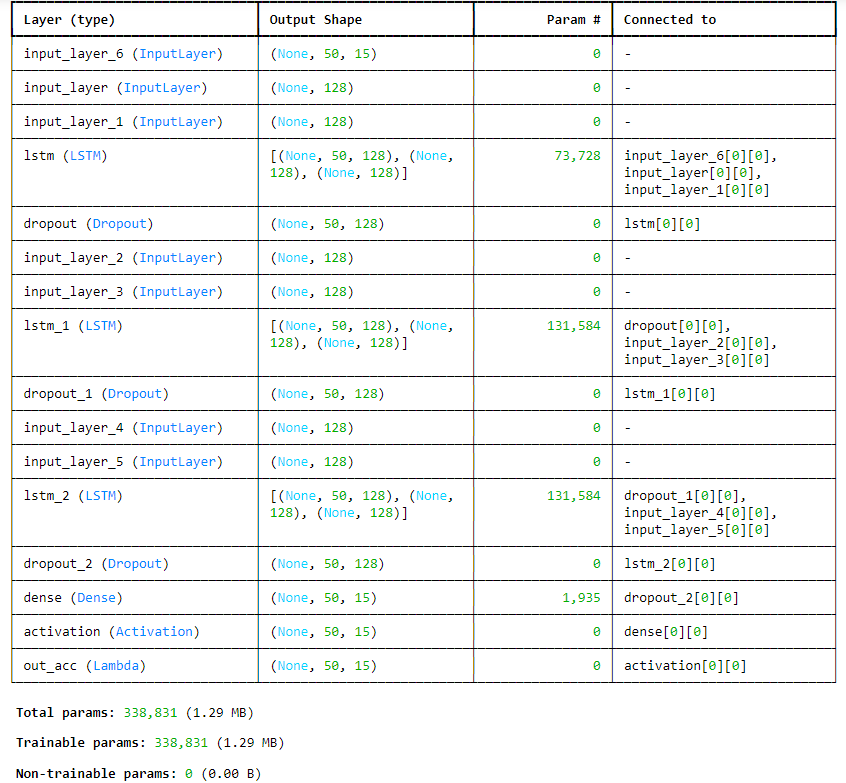
\includegraphics[width=\textwidth]{lstm_architecutre.png}
\caption{LSTM Network Architecture} \label{fig1}
\end{figure}


Below, I provide a detailed justification for each element incorporated into the model:

\begin{enumerate}
\item \textbf{Multiple Input Layers}: To handle various streams of data simultaneously, essential for complex sequences like game levels. This allows the network to process different types of information concurrently, improving its ability to learn intricate patterns and relationships within the data.\\

\item \textbf{LSTM Layers}: Core of the network, enabling it to learn temporal dependencies and generate coherent sequences. Long Short-Term Memory (LSTM) networks are particularly suited for sequential data as they can maintain long-term dependencies and are robust against vanishing gradient issues, which are common in standard RNNs.\\

\item \textbf{Dropout Layers}: Prevent overfitting by randomly dropping units during training. This regularization technique helps the network generalize better by not relying too heavily on any single node, thus enhancing its performance on unseen data.\\

\item \textbf{Dense Layer}: Aggregates the learned features and makes the final predictions. This layer consolidates the information extracted by the LSTM layers and maps it to the output space, making it essential for the final decision-making process.\\

\item \textbf{Activation Layer}: Ensures that the output values are within a specific range, necessary for classification tasks. For instance, using a softmax activation function in the final layer converts the network's outputs into probability distributions, facilitating the prediction of categorical outcomes.\\

\item \textbf{Lambda Layer}: A custom layer for specific processing or transformations. This layer can be used to implement custom operations that are not covered by standard Keras layers, allowing for greater flexibility in defining the network architecture.\\
\end{enumerate}


To evaluate the performance of the model, we employed various validation metrics during the experiments. These metrics provide insights into how well the model is learning and generalizing from the training data. The primary metric used for validation was the custom accuracy (custom\_acc), which measures the model's ability to correctly predict the next character in the sequence.

During training, we monitored the following metrics:

\begin{enumerate}
\item \textbf{Training Loss}: The loss function value computed on the training data, indicating how well the model is fitting the training data.\\

\item \textbf{Validation Loss}: The loss function value computed on the validation data, providing an indication of how well the model is generalizing to unseen data.\\

\item \textbf{Training Accuracy}: The accuracy of the model on the training data.\\

\item \textbf{Validation Accuracy}: The accuracy of the model on the validation data.\\
\end{enumerate}

The training process included early stopping with a patience of 20 epochs, meaning that if the validation accuracy did not improve for 20 consecutive epochs, the training would stop early. This mechanism is crucial for preventing overfitting and ensuring that the model does not learn noise from the training data.



\section{Experiment}
In this section, I will showcase the experiments done for my research. The experiment is similar to Summerville, A., \& Mateas, M. (2016)~\cite{ref_article14} work, with some changes suggested by Zhihan Yang (2020)\cite{ref_article30}. The experiment aims to replicate the generation of Super Mario levels as strings using LSTM networks. However, there are deviations from the original implementation described in the paper:

\begin{enumerate}

\item Snaking and level depth are not utilized in this implementation. The paper suggests adjusting the number of characters between the left and right sides of pipes by snaking down and up, but this approach is not adopted here as it can lead to inefficiency.

\item The method of adding depth characters to columns is reconsidered. Instead of appending depth characters to later columns, which may lead to inefficiency given the limited sequence length, an alternative approach is explored.

\item Validation is conducted after each epoch in this implementation, contrary to the paper's suggestion of validation after every 200 training examples. This decision was made for clarity and simplicity of the experiment setup.

\item The achievement of perfect pipe generation is not realized in this implementation.

\end{enumerate}

My research aims to find out how changing the hyper-parameter values affects the quality and overall playability of the generated Super Mario Bros. levels. During my research I have conducted 19 experiments where I explored the effects of changing three of my hyper-parameters: number of epochs, learning rate, and the batch size. For the number of epochs I have chosen the values of 10 and 20, and an additional experiment where the number of epochs was 27. For the learning rate, I chose the values 1e-3, 2e-3, and 5e-3. And for the batch size, I experimented with the values 50, 100, and 200. Creating a model with every possible value combinations, I had a total of 18 trainings to complete, and an additional training where I trained the model on 27 epochs, with a learning rate of 5e-3 and a batch size of 100 (see Table 1).


\begin{table}
\centering
\begin{tabular}{|c|c|c|c|c|c|c|}
\hline
Model \# &  Epochs & Learning Rate & Batch Size & Training time & Val Loss & Val Acc\\
\hline
1 & 20 & 1e-3 & 50 & 5038,71 & 0,3187 & 0,9066\\
2 & 20 & 1e-3 & 100 & 4385,75 & 0,3072 & 0,9071\\
3 & 20 & 1e-3 & 200 & 4180,85 & 0,309 & 0,9048\\
4 & 20 & 2e-3 & 50 & 5454,67 & 0,331 & 0,906\\
5 & 20 & 2e-3 & 100 & 5098,4 & 0,3159 & 0,9078\\
6 & 20 & 2e-3 & 200 & 5263,9 & 0,3058 & 0,907\\
7 & 20 & 5e-3 & 50 & 6614,6 & 0,3462 & 0,9064\\
8 & 20 & 5e-3 & 100 & 6445,6 & 0,3387 & 0,9069\\
9 & 20 & 5e-3 & 200 & 6699,5 & 0,3208 & 0,9069\\
10 & 10 & 1e-3 & 50 & 3943,1 & 0,3019 & 0,9078\\
11 & 10 & 1e-3 & 100 & 3357,43 & 0,3051 & 0,9064\\
12 & 10 & 1e-3 & 200 & 3880,69 & 0,3316 & 0,899\\
13 & 10 & 2e-3 & 50 & 4083,59 & 0,3062 & 0,9077\\
14 & 10 & 2e-3 & 100 & 3575,59 & 0,3006 & 0,9069\\
15 & 10 & 2e-3 & 200 & 4390,27 & 0,3106 & 0,9042\\
16 & 10 & 5e-3 & 50 & 4842,43 & 0,3176 & 0,9079\\
17 & 10 & 5e-3 & 100 & 3638,49 & 0,3164 & 0,9067\\
18 & 10 & 5e-3 & 200 & 4932,08 & 0,3218 & 0,9014\\
19 & 27 & 5e-3 & 100 & 9553,62 & 0,3724 & 0,9047\\
\hline
\end{tabular}
\newline
\caption{Hyper-parameter values for each trained model.}\label{tab1}
\end{table}

All experiments were conducted using TensorFlow and Keras libraries on a machine with an Intel(R) Core(TM) i7-8665U CPU @ 1.90GHz 2.11 GHz processor and 16 GB of DDR3 RAM. The training data consisted of preprocessed Super Mario Bros. level data. The dataset used for training the LSTM networks was derived from The Video Game Level Corpus (VGLC)~\cite{ref_article16}, from which I used the total of 15 Super Mario Bros. levels and 22 Japanese Super Mario Brothers 2 levels. The levels had 16 unique characters (where each represented a specific tile from the game), and was preprocessed to sequences of length 50 for input into the model. The quality and playability of the generated levels were evaluated using a combination of qualitative assessments (e.g., visual inspection, playability testing) and quantitative metrics (e.g., completion rate, tile diversity).

Each training run followed a standardized procedure: the dataset was split into training and validation sets, the model was trained with specified hyper-parameters, and validation was conducted after each epoch. Models were saved after training for subsequent analysis.




\section{Results and Discussion}
The implementation I utilized\cite{ref_article30} offers several refinements over the original approach by Summerville and Mateas (2016)~\cite{ref_article14}, aiming to enhance both efficiency and clarity. The original methods, such as snaking sequences and column depth information, were designed to improve data locality and level progression understanding but could introduce complexity and inefficiency by doubling the dataset size and complicating the sequence structure. By not utilizing these techniques, my implementation avoids these inefficiencies, making the training process more straightforward and manageable. Additionally, instead of appending depth characters to sequences, which could be inefficient given the limited sequence length, I explored an alternative method for representing column depth information. This approach ensures the network remains efficient and focused on critical data aspects.

The original paper suggests frequent validation after every 200 tiles in the training sequence, which can fragment the evaluation process and not provide a comprehensive view of model performance. In contrast, my implementation conducts validation after each epoch, aligning with standard machine learning practices and offering a clearer, more consistent performance evaluation. This enhanced validation strategy simplifies the experiment setup, making it easier to manage and interpret results, thereby improving clarity and reproducibility.

While the original paper acknowledges the challenge of generating coherent vertical structures like pipes and suggests treating different parts of the pipe separately, perfect pipe generation was not achieved in this implementation either. However, by focusing on the overall coherence and playability of generated levels, this approach continues to address this challenge. This reflects an adaptive and iterative problem-solving strategy aimed at progressively improving game level generation.

The training time for each model was found to increase proportionally with the number of epochs and batch size. The most significant training time was observed in Training 19, which utilized 27 epochs and a batch size of 100. This result is expected as more epochs and larger batch sizes inherently require more computational resources and time to process the data (see Fig.~\ref{fig2}).

\begin{figure}
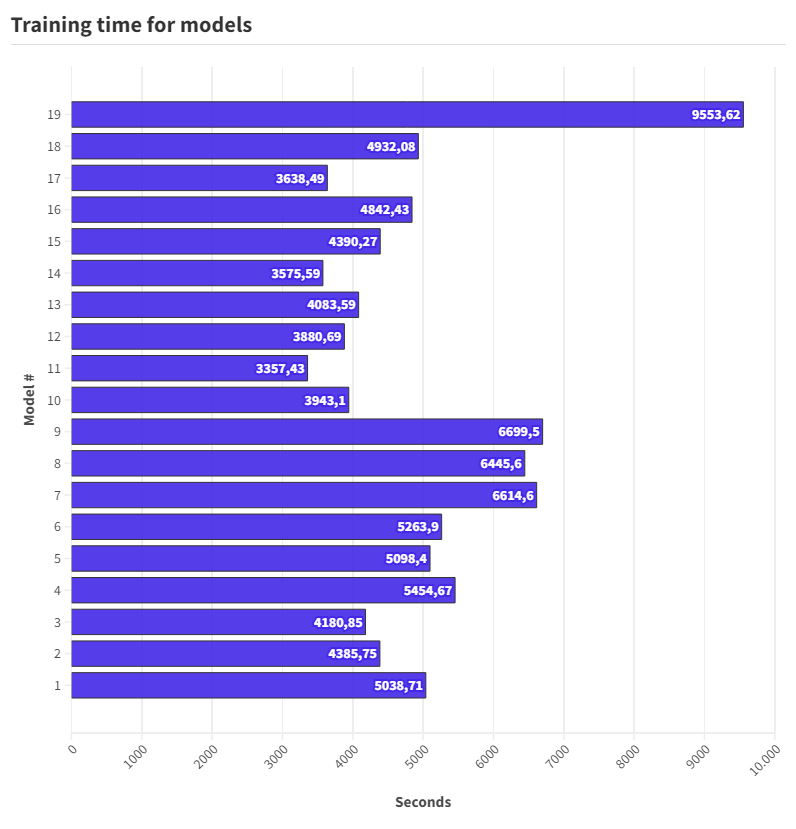
\includegraphics[width=\textwidth]{Training time for models (1).png}
\caption{Training time for each model} \label{fig2}
\end{figure}

Lower loss and validation loss values are indicative of better model performance. Among all the experiments, Training 19, with 27 epochs, a learning rate of 5e-3, and a batch size of 100, achieved the lowest loss. However, it is noteworthy that while higher learning rates (such as 5e-3) resulted in lower training losses (e.g., Trainings 7, 8, and 19) (see Fig.~\ref{fig3}), this did not consistently correlate with the lowest validation losses, suggesting potential overfitting or instability in model generalization.

\begin{figure}
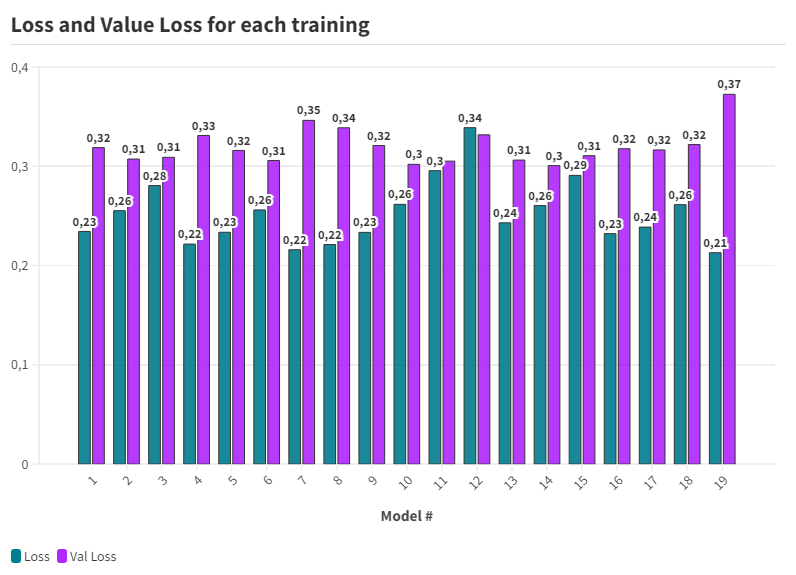
\includegraphics[width=\textwidth]{Loss and Value Loss for each training.png}
\caption{Loss and Value Loss for each training} \label{fig3}
\end{figure}

The highest training accuracy (Out Acc Custom Acc) achieved was 0.9323 in Training 19. Validation accuracy metrics were slightly lower but remained consistent with training accuracy across all experiments, indicating an absence of severe overfitting (see Fig.~\ref{fig4}). This consistency suggests that the models maintained their performance on unseen validation data, which is critical for reliable procedural content generation.

\begin{figure}
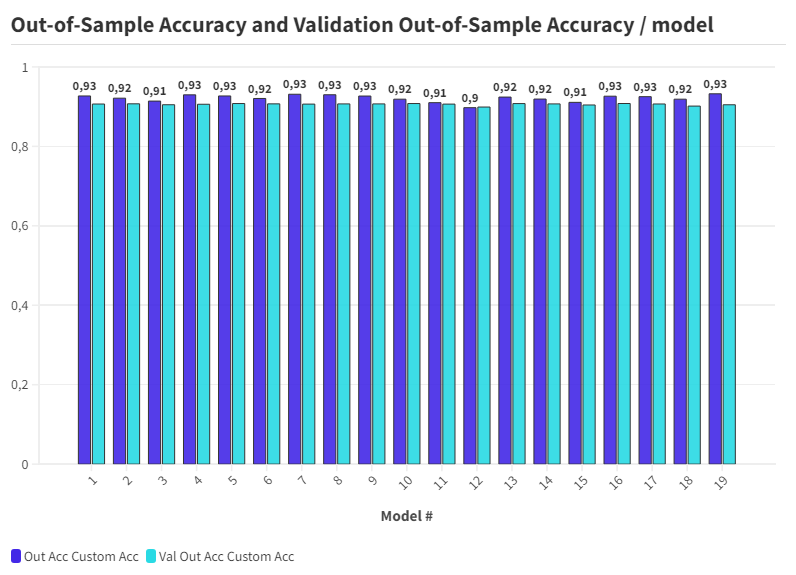
\includegraphics[width=\textwidth]{Out-of-Sample Accuracy and Validation Out-of-Sample Accuracy _ model.png}
\caption{Out-of-Sample Accuracy and Validation Out-of-Sample Accuracy / model} \label{fig4}
\end{figure}

The generated levels exhibited variability in the number of enemies and obstacles. Generally, models trained with 20 epochs produced levels with a higher number of enemies and obstacles. However, no clear correlation was observed between batch size and the number of enemies or obstacles. The number of obstacles remained relatively stable across different hyper-parameter settings, indicating that certain aspects of level design were less sensitive to changes in these parameters (see Fig.~\ref{fig5}).

\begin{figure}
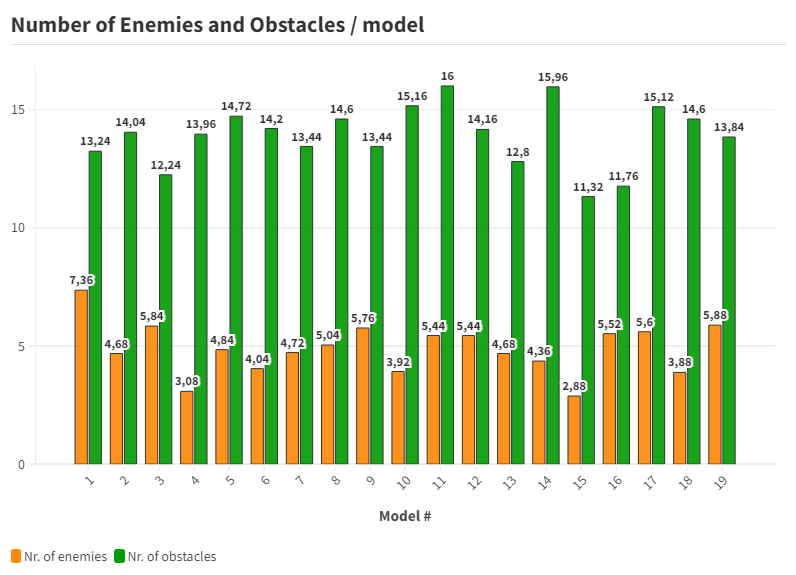
\includegraphics[width=\textwidth]{Number of Enemies and Obstacles _ model.png}
\caption{Number of Enemies and Obstacles / model} \label{fig5}
\end{figure}

Levels generated with 10 epochs were observed to be more flat and less detailed compared to those generated with 20 epochs. The latter generally produced more intricate and challenging levels, demonstrating the benefit of extended training for capturing more nuanced patterns and complexities in level design. Additionally, a learning rate of 5e-3 consistently yielded levels with higher complexity and detail, enhancing the overall playability and engagement of the generated content (see Fig.~\ref{fig6} and Fig.~\ref{fig7}).

\begin{figure}
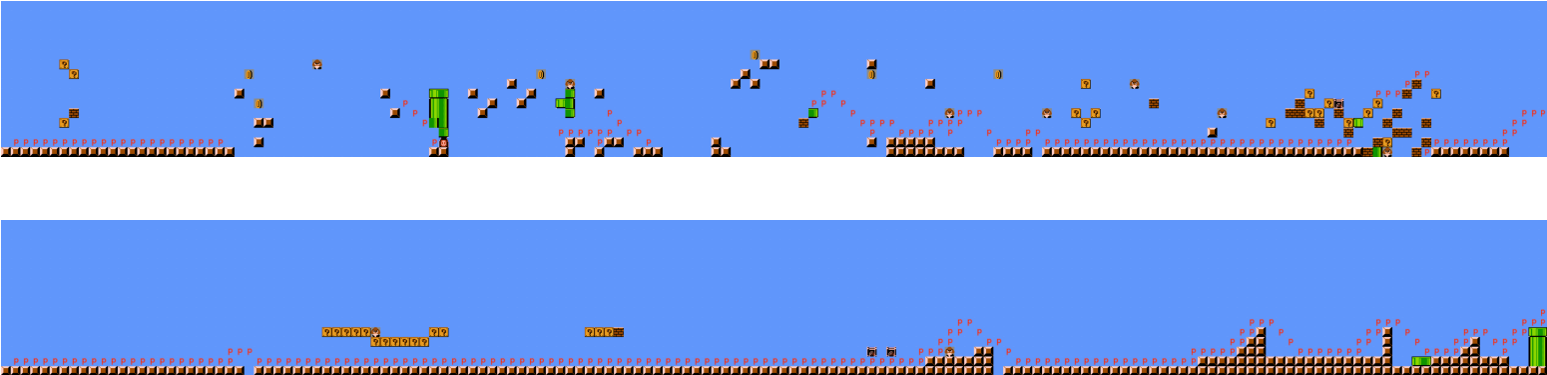
\includegraphics[width=\textwidth]{10_example.png}
\caption{Example of levels generated from models trained for 10 epochs} \label{fig6}
\end{figure}

\begin{figure}
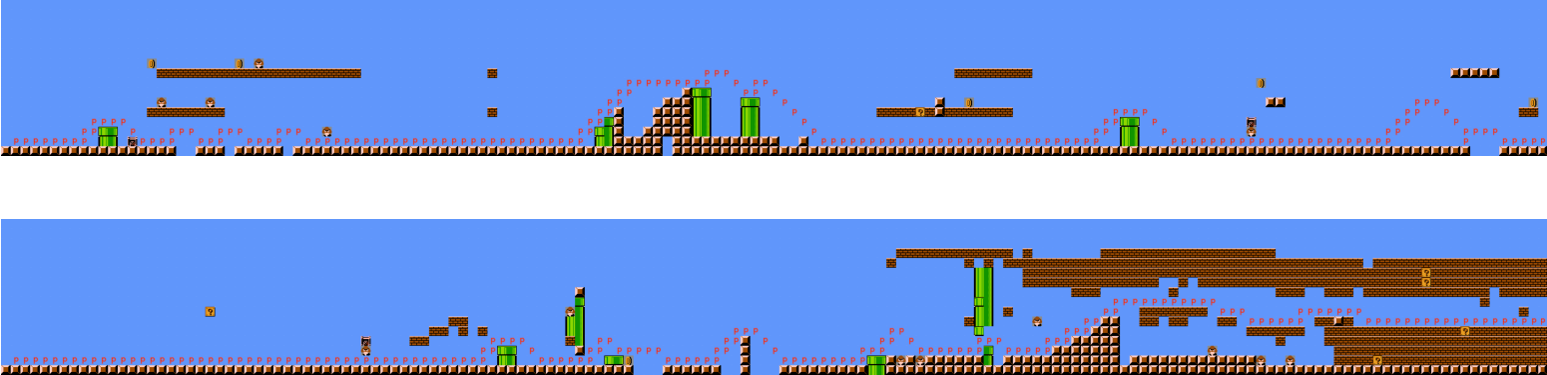
\includegraphics[width=\textwidth]{20_example.png}
\caption{Example of levels generated from models trained for 20 epochs} \label{fig7}
\end{figure}


The completeness of generated levels, defined as the percentage of levels that can be completed from start to finish, emerged as a crucial metric. Training 2, with 20 epochs, a learning rate of 1e-3, and a batch size of 100, achieved the highest completeness at 60\%. Interestingly, higher completeness percentages were often associated with levels featuring fewer enemies and obstacles. For instance, Training 15, with 10 epochs, a learning rate of 2e-3, and a batch size of 200, also showed high completeness (60\%) while generating the fewest enemies (2.88) and a moderate number of obstacles (11.32) (see Fig.~\ref{fig8}).

\begin{figure}
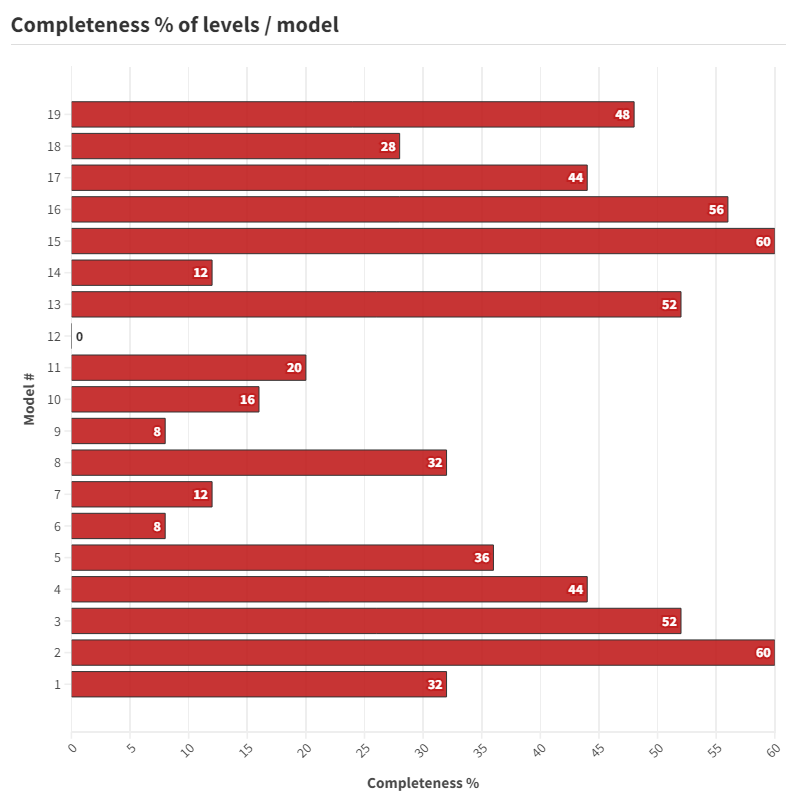
\includegraphics[width=\textwidth]{Completeness percentage of levels _ model.png}
\caption{Completeness \% of levels / model} \label{fig8}
\end{figure}

The decision to limit the training to 27 epochs, despite initially specifying 30 or 50 epochs, is primarily driven by the principle of early stopping, which is a crucial aspect of my experimentation setup. Early stopping is a technique used to prevent overfitting and improve the generalization of the model by halting training when the model's performance on the validation set stops improving. In my implementation, I employed an early stopping callback with a patience parameter set to 20 epochs. This means that if the model's performance on the validation set does not improve for 20 consecutive epochs, the training process is automatically stopped. In both instances where I specified 30 and 50 epochs, the training was halted at 27 epochs because the early stopping criteria were met. This indicates that the model reached a point where further training did not lead to better validation performance, suggesting that the optimal weights had already been achieved. Continuing the training beyond this point would likely result in overfitting, where the model starts to learn noise in the training data rather than meaningful patterns, thus degrading its performance on unseen data.

Upon comparing the training processes with 27 epochs and 20 epochs, using a batch size of 100 and a learning rate of 5e-3, several observations can be made regarding their performance and behavior based on the provided validation loss and accuracy metrics.

In the initial epochs, both Training \#19 and Training \#8 exhibit a significant drop in validation loss. This is expected as the model starts to learn from the data. During epochs 1 to 10, Training \#19 generally shows slightly lower validation loss compared to Training \#8. For example, at epoch 2, Training \#19 has a validation loss of 0.3276 while Training \#8 has 0.3665. This trend continues through the initial epochs, indicating potentially more effective learning in Training \#19. After about epoch 10, the validation loss for both trainings stabilizes, with minor fluctuations. The loss values between the two trainings converge around similar ranges (0.3 to 0.34), suggesting that the network has reached a plateau in learning efficiency. By epoch 20, Training \#19 and Training \#8 both exhibit validation losses in the range of 0.34 to 0.35. Training \#19 continues to 27 epochs, but the loss does not show significant improvement, indicating diminishing returns for further epochs (see Fig.~\ref{fig9}).

\begin{figure}
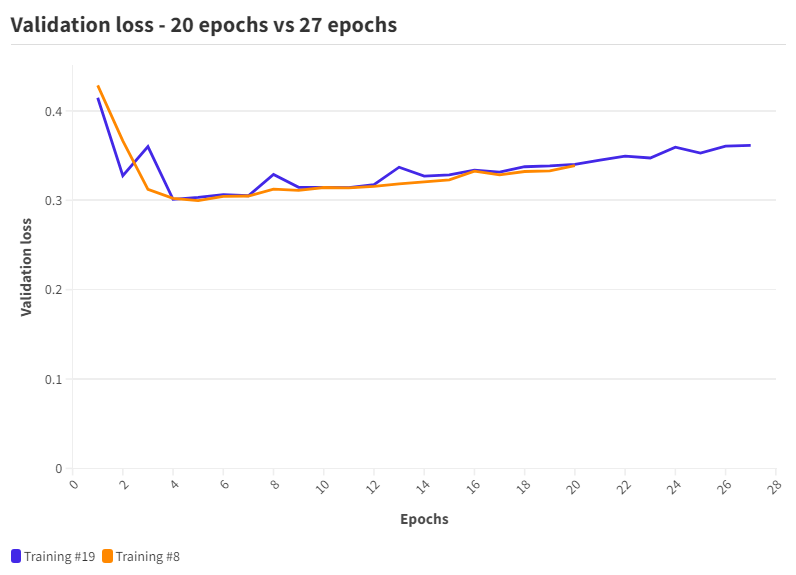
\includegraphics[width=\textwidth]{val loss.png}
\caption{Validation loss - 20 epochs vs 27 epochs} \label{fig9}
\end{figure}


In terms of validation accuracy, both trainings show substantial improvements in the early epochs. For instance, Training \#19 goes from 0.8634 at epoch 1 to over 0.9 by epoch 4, and Training \#8 shows a similar trend. During epochs 1 to 10, Training \#19 generally maintains slightly higher validation accuracy compared to Training \#8. For example, at epoch 10, Training \#19 has a validation accuracy of 0.9064 compared to Training \#8's 0.9078. Both trainings see stabilization in accuracy values after the initial learning phase, consistently staying above 0.90. The accuracy remains relatively constant with minor fluctuations. Beyond 20 epochs, the accuracy does not show notable improvement for Training \#19, maintaining around 0.905 to 0.907. This indicates that additional training epochs did not significantly enhance the model's predictive performance(see Fig.~\ref{fig10}).

\begin{figure}
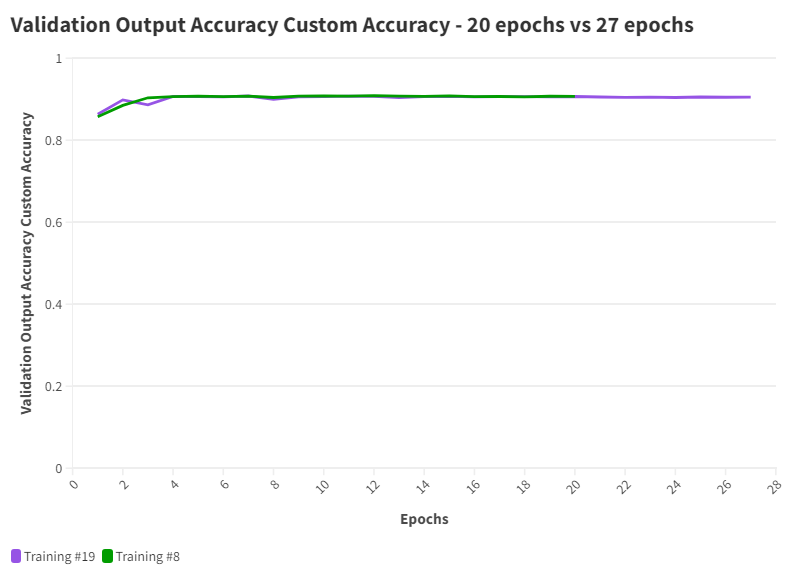
\includegraphics[width=\textwidth]{val acc.png}
\caption{Validation Output Accuracy Custom Accuracy - 20 epochs vs 27 epochs} \label{fig10}
\end{figure}


Based on these observations, extending the training to 27 epochs instead of stopping at 20 did not yield significant improvements in validation loss or accuracy. Both metrics show stabilization and diminishing returns with additional epochs. Therefore, 20 epochs might be a more efficient choice, balancing training time and performance. The decision to stop at 27 epochs in this context is reasonable but does not necessarily provide additional benefits compared to stopping at 20 epochs, suggesting that the optimal number of epochs might lie closer to 20. Exploring higher numbers of epochs might provide more insights into the model's performance limits and whether a more extended training period can yield any incremental improvements.


The optimal hyper-parameters for generating high-quality and playable levels were identified as follows: 20 epochs, a learning rate of 1e-3, and a batch size of 100 (Training 2). This configuration provided a balanced approach, achieving high completeness while maintaining favorable accuracy and validation metrics. Training 15 also proved effective, demonstrating that fewer epochs can still yield excellent results with appropriate tuning of learning rate and batch size. There are evident trade-offs between the number of epochs and training time. While more epochs generally lead to improved performance metrics, the associated increase in training time is substantial. Furthermore, although a higher learning rate (5e-3) facilitated lower training loss values, this did not necessarily translate to better completeness percentages, highlighting the complexity of optimizing hyperparameters. Consistency in generating playable levels is more critical than achieving the lowest possible loss values. Models with lower loss and high accuracy (e.g., Training 19) did not always produce the highest completeness percentages. Additionally, the variability in the number of enemies and obstacles suggests that increased epochs help stabilize the level generation process, reducing drastic differences in generated content.


\section{Conclusion}
The research conducted on procedural content generation for Super Mario Bros. levels using Long Short-Term Memory (LSTM) networks provides valuable insights into the effects of hyper-parameters on model performance and the quality of generated levels. By systematically varying the number of epochs, learning rate, and batch size, I have identified optimal settings that balance model accuracy, training efficiency, and level playability. To further improve the quality and controllability of generated levels, future research could explore additional hyper-parameter settings and incorporate other advanced techniques, such as reinforcement learning and more complex network architectures. Experimentation with different game genres and the integration of user feedback into the generation process could also improve the applicability and robustness of procedural content generation methods.

In conclusion, this research demonstrates the potential of LSTM networks in procedural content generation, providing a framework for optimizing hyper-parameters to achieve high-quality, playable levels. The findings contribute to the broader field of AI-driven game design, offering practical insights and tools that can benefit game developers, researchers, and educators alike.

\begin{thebibliography}{8}

\bibitem{ref_article1}
González-Hermida, M., Costa-Montenegro, E., Legerén-Lago, B., \& Pena-Gimenez, A. (2020). Study of Artificial Intelligent Algorithms Applied in Procedural Content Generation in Video Games. Eludamos: Journal for Computer Game Culture

\bibitem{ref_article2}
Mott, J., Nandi, S., \& Zeller, L. (2019). Controllable and Coherent Level Generation: A Two-Pronged Approach, Proceeding of EXAG at 15th AAAI conference.

\bibitem{ref_article3}
Barriga, N. A. (2019, March). A Short Introduction to Procedural Content Generation Algorithms for Videogames. International Journal on Artificial Intelligence Tools, 28(02), 1930001. https://doi.org/10.1142/s0218213019300011

\bibitem{ref_article4}
Roberts, J., \& Chen, K. (2013, August 29). Learning-Based Procedural Content Generation. arXiv.org. https://arxiv.org/abs/1308.6415

\bibitem{ref_article5}
Volz, V., Justesen, N., Snodgrass, S., Asadi, S., Purmonen, S., Holmgård, C., Togelius, J., Risi, S. (2020). Capturing Local and Global Patterns in Procedural Content Generation via Machine Learning. IEEE Conference on Games, CoG 2020, Osaka, Japan, August 24-27, 2020, 399–406. doi:10.1109/COG47356.2020.9231944

\bibitem{ref_article6}
Baron, J. R. (2017). Procedural Dungeon Generation Analysis and Adaptation. Proceedings of the 2017 ACM Southeast Regional Conference, Kennesaw, GA, USA, April 13-15, 2017, 168–171. doi:10.1145/3077286.3077566

\bibitem{ref_article7}
Blatz, M., \& Korn, O. (2017). A Very Short History of Dynamic and Procedural Content Generation. In O. Korn \& N. Lee (Eds.), Game Dynamics: Best Practices in Procedural and Dynamic Game Content Generation (pp. 1–13). doi:10.1007/978-3-319-53088-8\_1

\bibitem{ref_article8}
R. van der Linden, R. Lopes and R. Bidarra, "Procedural Generation of Dungeons," in IEEE Transactions on Computational Intelligence and AI in Games, vol. 6, no. 1, pp. 78-89, March 2014, doi: 10.1109/TCIAIG.2013.2290371

\bibitem{ref_article9}
Julian Togelius, Emil Kastbjerg, David Schedl, and Georgios N. Yannakakis. 2011. What is procedural content generation? Mario on the borderline. In Proceedings of the 2nd International Workshop on Procedural Content Generation in Games (PCGames '11). Association for Computing Machinery, New York, NY, USA, Article 3, 1–6. https://doi.org/10.1145/2000919.2000922

\bibitem{ref_article10}
Risi, S., \& Togelius, J. (2019, November 29). Increasing Generality in Machine Learning through Procedural Content Generation. arXiv.org. https://arxiv.org/abs/1911.13071

\bibitem{ref_article11}
Chen, E., Sydora, C., Burega, B., Mahajan, A., Abdullah, A., Gallivan, M., \& Guzdial, M. (2020, October 1). Image-to-Level: Generation and Repair. Proceedings of the AAAI Conference on Artificial Intelligence and Interactive Digital Entertainment. https://doi.org/10.1609/aiide.v16i1.7429

\bibitem{ref_article12}
Guzdial, M., Liao, N., \& Riedl, M. (2018, September 25). Co-Creative Level Design via Machine Learning. arXiv.org. https://arxiv.org/abs/1809.09420

\bibitem{ref_article13}
Volkmar, G., Mählmann, N., Malaka, R. (2019). Procedural Content Generation in Competitive Multiplayer Platform Games. In: van der Spek, E., Göbel, S., Do, EL., Clua, E., Baalsrud Hauge, J. (eds) Entertainment Computing and Serious Games. ICEC-JCSG 2019. Lecture Notes in Computer Science(), vol 11863. Springer, Cham. https://doi.org/10.1007/978-3-030-34644-7\_18

\bibitem{ref_article14}
Summerville, A., \& Mateas, M. (2016, March 2). Super Mario as a String: Platformer Level Generation Via LSTMs. arXiv.org. https://arxiv.org/abs/1603.00930

\bibitem{ref_article15}
A. Zafar, S. Hassan and Q. S. uddin, "Corpus for Angry Birds Level Generation," 2019 2nd International Conference on Computing, Mathematics and Engineering Technologies (iCoMET), Sukkur, Pakistan, 2019, pp. 1-4, doi: 10.1109/ICOMET.2019.8673443

\bibitem{ref_article16}
Summerville, A. J., Snodgrass, S., Mateas, M., \& Ontañón, S. (2016, June 23). The VGLC: The Video Game Level Corpus. arXiv.org.https://arxiv.org/abs/1606.07487

\bibitem{ref_article17}
X. Neufeld, S. Mostaghim and D. Perez-Liebana, "Procedural level generation with answer set programming for general Video Game playing," 2015 7th Computer Science and Electronic Engineering Conference (CEEC), Colchester, UK, 2015, pp. 207-212, doi: 10.1109/CEEC.2015.7332726

\bibitem{ref_article18}
Snodgrass, S., Summerville, A., \& Ontañón, S. (2021, June 25). Studying the Effects of Training Data on Machine Learning-Based Procedural Content Generation. Proceedings of the AAAI Conference on Artificial Intelligence and Interactive Digital Entertainment. https://doi.org/10.1609/aiide.v13i1.12930

\bibitem{ref_article19}
Smelik, R. M., Kraker, K. J. de, Groenewegen, S. A., Tutenel, T., \& Bidarra, R. (2009, June). A survey of procedural methods for terrain modelling. Proceedings of the CASA’09 Workshop on 3D Advanced Media in Gaming and Simulation, 25–34. Retrieved from http://graphics.tudelft.nl/Publications-new/2009/SDGTB09a

\bibitem{ref_article20}
Stefan Greuter, Jeremy Parker, Nigel Stewart, and Geoff Leach. 2003. Real-time procedural generation of `pseudo infinite' cities. In Proceedings of the 1st international conference on Computer graphics and interactive techniques in Australasia and South East Asia (GRAPHITE '03). Association for Computing Machinery, New York, NY, USA, 87–ff. https://doi.org/10.1145/604471.604490

\bibitem{ref_article21}
M. Werneck and E. W. G. Clua, "Generating Procedural Dungeons Using Machine Learning Methods," 2020 19th Brazilian Symposium on Computer Games and Digital Entertainment (SBGames), Recife, Brazil, 2020, pp. 90-96, doi: 10.1109/SBGames51465.2020.00022

\bibitem{ref_article22}
Ammanabrolu, P., Cheung, W., Tu, D., Broniec, W., \& Riedl, M. O. (2020, January 28). Bringing Stories Alive: Generating Interactive Fiction Worlds. arXiv.org. https://arxiv.org/abs/2001.10161

\bibitem{ref_article23}
Panagiotou, E., \& Charou, E. (2020, October 13). Procedural 3D Terrain Generation using Generative Adversarial Networks. arXiv.org. https://arxiv.org/abs/2010.06411

\bibitem{ref_article24}
López, C. E., Cunningham, J., Ashour, O., and Tucker, C. S. (June 3, 2020). "Deep Reinforcement Learning for Procedural Content Generation of 3D Virtual Environments." ASME. J. Comput. Inf. Sci. Eng. October 2020; 20(5): 051005. https://doi.org/10.1115/1.4046293

\bibitem{ref_article25}
Summerville, A., Snodgrass, S., Guzdial, M., Holmgård, C., Hoover, A. K., Isaksen, A., Nealen, A., \& Togelius, J. (2017, February 2). Procedural Content Generation via Machine Learning (PCGML). arXiv.org. https://arxiv.org/abs/1702.00539

\bibitem{ref_article26}
Gisslén, L., Eakins, A., Gordillo, C., Bergdahl, J., \& Tollmar, K. (2021, March 8). Adversarial Reinforcement Learning for Procedural Content Generation. arXiv.org. https://arxiv.org/abs/2103.04847

\bibitem{ref_article27}
Khalifa, A., Bontrager, P., Earle, S., \& Togelius, J. (2020, January 24). PCGRL: Procedural Content Generation via Reinforcement Learning. arXiv.org. https://arxiv.org/abs/2001.09212

\bibitem{ref_article28}
Liang, Y., Li, W., Ikeda, K. (2019). Procedural Content Generation of Rhythm Games Using Deep Learning Methods. In: van der Spek, E., Göbel, S., Do, EL., Clua, E., Baalsrud Hauge, J. (eds) Entertainment Computing and Serious Games. ICEC-JCSG 2019. Lecture Notes in Computer Science(), vol 11863. Springer, Cham. https://doi.org/10.1007/978-3-030-34644-7\_11

\bibitem{ref_article29}
Jadhav, M., \& Guzdial, M. (2021, October 4). Tile Embedding: A General Representation for Level Generation. Proceedings of the AAAI Conference on Artificial Intelligence and Interactive Digital Entertainment. https://doi.org/10.1609/aiide.v17i1.18888

\bibitem{ref_article30}
Zhihan Y. 2020. Generating Super Mario levels using LSTM.
https://github.com/zhihanyang2022/super\_mario\_as\_a\_string?tab=readme-ov-file. (2024)


\end{thebibliography}
\end{document}

